%!TEX TS-program = xelatex
\documentclass[]{vella-cv}
\usepackage{afterpage}
\usepackage{hyperref}
\usepackage{color}
\usepackage{xcolor}
\usepackage{smartdiagram}
\usepackage{fontspec}
% if you want to add fontawesome package
% you need to compile the tex file with LuaLaTeX
% References:
%   http://texdoc.net/texmf-dist/doc/latex/fontawesome/fontawesome.pdf
%   https://www.ctan.org/tex-archive/fonts/fontawesome?lang=en
%\usepackage{fontawesome}
\usepackage{metalogo}
\usepackage{dtklogos}
\usepackage[utf8]{inputenc}
\usepackage{tikz}
\usetikzlibrary{mindmap,shadows}
\hypersetup{
    pdftitle={},
    pdfauthor={},
    pdfsubject={},
    pdfkeywords={},
    colorlinks=false,           % no lik border color
    allbordercolors=white       % white border color for all
}
\smartdiagramset{
    bubble center node font = \footnotesize,
    bubble node font = \footnotesize,
    % specifies the minimum size of the bubble center node
    bubble center node size = 0.5cm,
    %  specifies the minimum size of the bubbles
    bubble node size = 0.5cm,
    % specifies which is the distance among the bubble center node and the other bubbles
    distance center/other bubbles = 0.3cm,
    % sets the distance from the text to the border of the bubble center node
    distance text center bubble = 0.5cm,
    % set center bubble color
    bubble center node color = pblue,
    % define the list of colors usable in the diagram
    set color list = {lightgray, materialcyan, orange, green, materialorange, materialteal, materialamber, materialindigo, materialgreen, materiallime},
    % sets the opacity at which the bubbles are shown
    bubble fill opacity = 0.6,
    % sets the opacity at which the bubble text is shown
    bubble text opacity = 0.5,
}

\addbibresource{bibliography.bib}
\RequirePackage{xcolor}
\definecolor{pblue}{HTML}{0395DE}

\begin{document}
\header{Lex}{Vella}
      {Systems Administrator}
      
% Fake text to add separator      
\fcolorbox{white}{gray}{\parbox{\dimexpr\textwidth-2\fboxsep-2\fboxrule}{%
.....
}}

% In the aside, each new line forces a line break
\begin{aside}
  
\includegraphics[scale=0.15]{img/resumepic.png}
  \section{Address}
    The Castle
    Vancouver, BC
    ~
  \section{Tel \& Skype}
    +1 323 275 1323
    lexvella
    ~
  \section{Mail}
    \href{mailto:lex@vella.io}{\textbf{lex@}vella.io}
    ~
  \section{Web \& Git}
    \href{http://vella.io}{vella.io}
    \href{https://bitbucket.org/lexvella}{bitbucket.org/lexvella}
    \href{https://github.com/lexvella}{github.com/lexvella}
    ~
  % use  \hspace{} or \vspace{} to change bubble size, if needed
  \section{Programming}
    \smartdiagram[bubble diagram]{
        \textbf{Lisp},
        \textbf{Python},
        \textbf{SQL},
        \textbf{Clojure\vspace{3mm}},
        \textbf{HTML/CSS}\\\textbf{JS/jQuery},
        \textbf{Powershell},
        \textbf{Android},
        \textbf{Bash}
    }
    ~
    ~
    ~
  \section{Personal Skills}
    \smartdiagram[bubble diagram]{
        \textbf{Team}\\\textbf{Leader},
        \textbf{Initiative},
        \textbf{Communicator},
        \textbf{Curiosity},
        \textbf{Independent},
        \textbf{\vspace{2mm}Manage\vspace{2mm}},
        \textbf{Organize}
    }
    ~
\end{aside}
~
\section{Experience}
\begin{entrylist}
  \entry
    {01/14 - Now}
    {Sr. Systems Administrator / DevOps Engineer}
    {Manluk Industries}
    {Successfully lead the Information Technology department of an automated robotic manufacturing corporation and several start up enterprises, with several hundred employees and four separate plants. Key duties included acting as a system, network, and business intelligence architect, as well as senior technician for the corporation. Automated operations and integrated systems with Python.\\\\
    \emph{Virtualized existing backend Windows and Unix infrastructure to provisioned virtual machines running on VMWare ESXi and Xen hosts, managed through a Saltstack Master\\\\}
    \emph{Architect of the successful deployment of a complete migration of critical infrastructure, including our ERP, Exchange, PBX, databases, and business process systems to a full hybrid cloud running through Amazon Web Service’s EC2, S3, SES/SNS, Route 53, CloudFormation and Elastic Beanstalk\\\\}
    \emph{Modernized and overhauled corporate policies, strategic direction, and data culture, including the push to hybrid cloud services, real-time data collection, a teleworkers initiative, and security\\}}
    \entry
    {06/12 - 11/14}
    {Intelligence Operator}
    {Canadian Forces}
    {Employed by the Canadian Forces as an infantry soldier, and then later in my contract, reassigned to an Edmonton based Military Intelligence unit per Component Transfer. Systems and Networking related duties at this time involved securing internal communications for field operations.\\}
    \entry
    {11/14 - Now}
    {Freelancer / Founder}
    {AlephZero Consulting}
    {Founded a consulting company immediately after leaving the Canadian Forces. We provide expert system administration, system design, and support to local startups.\\}
    \entry
    {12/09 - 06/10}
    {Project Manager}
    {MV Faranda}
    {Project Manager for restoration of MV Faranda, an historic wooden yacht in BC, presently anchored in Oak Bay Marina}
\end{entrylist}

\section{Education}
\\\\
\begin{entrylist}
  \entry
    {2010}
    {Biochemistry and Computer Science}
    {University of Victoria}
    {Biochemistry, Physics, combined double major. Coursework in Software Development and Computer Networking.\\\\}
    \entry
    {2016}
    {B.Sc Computer Science and Information Systems}
    {Athabasca University}
    {Completing coursework via correspondence}
\end{entrylist}

\newpage

\begin{aside}
~
~
~
  \section{OS Preference}
    \textbf{GNU/Linux}
\includegraphics[scale=0.40]{img/5stars.png}
    \textbf{Unix}
\includegraphics[scale=0.40]{img/4stars.png}
    \textbf{MacOS}
\includegraphics[scale=0.40]{img/4stars.png}
    \textbf{Windows}
\includegraphics[scale=0.40]{img/3stars.png}
    ~
  \section{Cities Lived}
    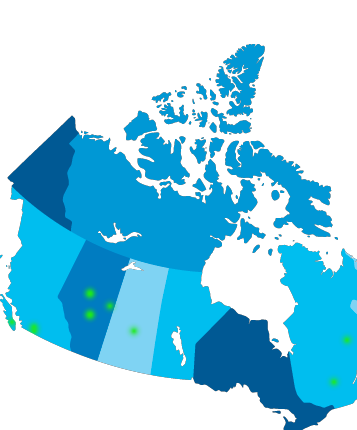
\includegraphics[scale=0.25]{img/canadaresidences.png}
    ~
  \section{Languages}
    \textbf{French}
\includegraphics[scale=0.40]{img/3stars.png}
    \textbf{English}
\includegraphics[scale=0.40]{img/5stars.png}
    ~
\end{aside}

\section{Internships}
Moli Energy, Maple Ridge, 2008\\
\textbf{Worked as an intern at Moli Energy Canada investigating potential use cases for Molybdenum based battery technology as an alternative to lithium.}\\
\emph{Also provided IT support for the on site research and development team.}
\\
\section{Honors \& Awards}
\begin{entrylist}
  \entry
    {10/12}
    {Platoon Marksmanship Award}
    {Canadian Forces}
    {CF-BMQ St Jean Sur Richelieu.\\
    \emph{C7 Rifle Range}}
\end{entrylist}

\section{Certifications}
\begin{entrylist}
  \entry
    {04/13}
    {Introductory Python}
    {Coursera + University of Michigan E-learning}
    {\emph{Building a Python Search Engine}}\\
    \entry
    {12/12}
    {St. John's First Aid}
    {Canadian Forces}
    {\emph{First responder for tourniquets, seizures, common wounds and trauma\\}}
    \entry
    {03/10}
    {MCSE}
    {Microsoft}
    {\emph{Expired}}\\
\end{entrylist}
\section{Volunteer Work}
\begin{entrylist}
  \entry
    {11/12 - 01/13}
    {Mustard Seed Food Bank}
    {Victoria, BC}
    {\emph{Provided food and household items to those in need\\}}
    \entry
    {09/07 - 04/08}
    {Pitt Meadows Volunteer Fire Department}
    {Pitt Meadows, BC}
    {\emph{Trainee volunteer firefighter}}

    
\end{entrylist}
\section{Errata}
Some notes about myself:\\
\emph{In my free time, I record music. My current tech projects include hacking at Lisp, and switching my editor from vim to emacs. My focus as a Systems Administrator tends toward penetration testing and an innate drive for network security. I'm currently working on my CISSP certifications, several courses on machine learning through Coursera, and taking mathematics courses through correspondence. I consider myself a fairly straight-forward, dyed-in-the-wool sysadmin. I prefer to be contacted initially via email.}
\\
\begin{flushleft}
\emph{July 5th, 2016}
\end{flushleft}
\begin{flushright}
\emph{Lex Vella}
\end{flushright}

\end{document}
